\documentclass{article}

\usepackage{polski}
\usepackage[UTF8]{inputenc}
\usepackage{graphicx}
\usepackage{float}
\usepackage[margin=1in]{geometry}
\usepackage{graphicx}
\usepackage{amsmath}
\usepackage{mathtools}
\usepackage{amssymb}
\usepackage{multirow}
\usepackage{changepage}

\title{Sprawozdanie}
\begin{document}

\begin{center}
\bgroup
\def\arraystretch{1.5}
\begin{tabular}{|c|c|c|c|c|c|}
	\hline
	EAIiIB & \multicolumn{2}{|c|}{\begin{tabular}{@{}c@{}}Autor 1 \\ Autor 2\end{tabular}} & Rok II & Grupa 5 & Zespół 6 \\
	\hline
	\multicolumn{3}{|c|}{\begin{tabular}{c}Temat: \\ Wahadło fizyczne \end{tabular}} & 
	\multicolumn{3}{|c|}{\begin{tabular}{c}Numer ćwiczenia: \\ 1 \end{tabular}} \\
	\hline
	Data wykonania & Data oddania & Zwrot do poprawki & Data oddania & Data zaliczenia & Ocena \\[8ex]
	\hline
\end{tabular}
\egroup
\end{center} 

%WSTEP
\section{Cel ćwiczenia}
Zapoznanie się z ruchem drgającym wahadła fizycznego. Wyznaczenie momentu bezwładności brył sztywnych przez pomiar okresu drgań.

\section{Wstęp teoretyczny}
\subsection{Wahadło fizyczne}
Wahadłem fizycznym nazywamy bryłę sztywną mogącą się obracać wokół osi obrotu $O$ nie przechodzącej przez środek ciężkości $S$. \\
\begin{figure}[!htb]
	\centering
	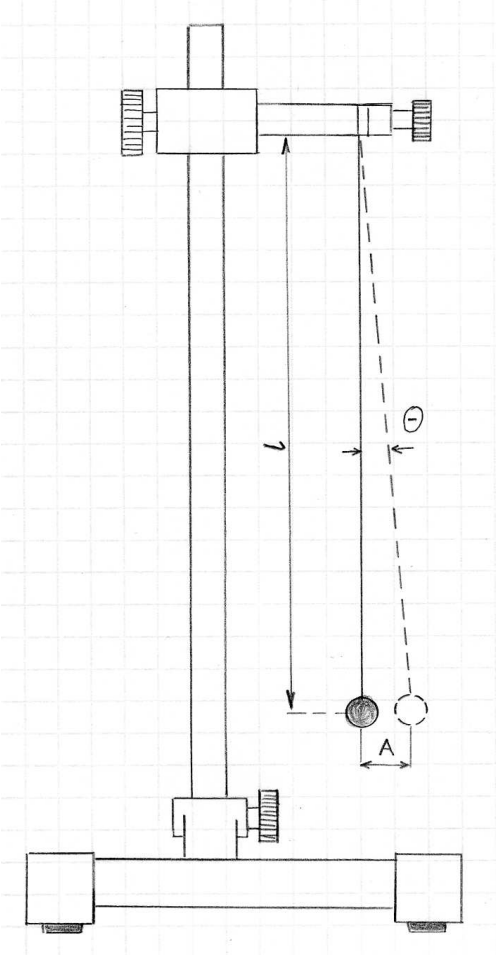
\includegraphics[scale=0.65]{wahadlo.png}
	\caption{Wahadło}
\end{figure}
\\
Wahadło odchylone od pionu o kąt $\Theta$, a następnie puszczone w swobodnie, będzie wykonywać drgania zwane ruchem wahadłowym. Dla wahadła fizycznego moment siły powstaje pod wpływem siły ciężkości.
\subsection{Moment bezwładności}
Moment bezwładności to miara bezwładności ciała w ruchu obrotowym. Im większy moment, tym trudniej zmienić ruch obrotowy ciała, np. rozkręcić dane ciało lub zmniejszyć jego prędkość obrotową. Moment bezwładności wyliczamy ze wzoru:
\begin{align*}
I = \sum_{i=1}^{n} m_{i}r_{i}^{2}
\end{align*}
\subsection{Definicja twierdzenia Steinera}
Moment bezwładności bryły sztywnej względem dowolnej osi jest równy sumie momentu bezwładności względem osi równoległej do danej i przechodzącej przez środek masy bryły oraz iloczynu masy bryły i kwadratu odległości między tymi dwiema osiami, co można wyrazić wzorem:
\begin{align}
I = I_{0} + md^{2} 
\end{align}

\subsection{Ruch harmoniczny}
To ruch okresowy, czyli ruch powtarzający się w regularnych odstępach czasu, w którym przemieszczenie x ciała zmienia się w funkcji czasu t w sposób sinusoidalny lub kosinusoidalny. Zależność przemieszczenia $x(t)$ ciała w ruchu harmonicznym opisuje poniższy wzór:
\begin{align}
 x(t) = A \cos (\omega t + \varphi)
\end{align}

W wahadle fizycznym, przy założeniu małego kąta odchylenia $\alpha$, prawdziwe jest następujące równanie:


\section{Ukłąd pomiarowy}
Zestaw ćwiczeniowy stanowi pręt, który zawiesza się na odpowiednim statywie, a następnie wprowadza w ruch drgający. Potrzebne przyrządy pomiarowe to waga elektroniczna, suwmiarka, przymiar milimetrowy oraz sekundomierz.
\begin{figure}[!htb]
	\centering
	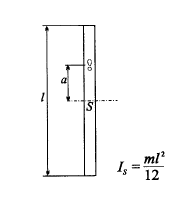
\includegraphics[scale=0.65]{pret.png}
	\caption{Pręt}
\end{figure}	
\section{Wykonanie ćwiczenia}
\begin{enumerate}
	\item Zmierzono masę pręta.
	\item Zmierzono rozmiary: pręta (l i a).
	\item Umieszczono pręt w statywie, wprowadzono go ruch drgający o amplitudzie nie przekraczającej kilku stopni i zmierzono czas 30 drgań.  Pomiar ten powtórzono dziesięciokrotnie.
\end{enumerate}
	

%KONIEC WSTEPU	

\pagebreak
\section{Opracowanie wyników}
\subsection{Obliczenia}
\begin{enumerate}
	\item Obliczamy moment bezwładności geometrycznie korzystając ze wzoru:
	$$ I_s = \frac{ml^2}{12} $$
	\item Wyznaczamy niepewność obliczonego momentu bezwładności w punkcie 1.
	\item Obliczamy moment bezwładności względem osi obrotu korzystając ze wzoru:
	$$T = 2 \pi  \sqrt{\frac{I_o}{mga}}$$
	\item Korzystając z twierdzenia Steinera obliczamy moment bezwładności względem osi przechodzącej przez środek masy.
	\item Wyznaczamy niepewność obliczonego momentu bezwładności w punkcie 4.
\end{enumerate}

\begin{figure}[!htb]
	\begin{adjustwidth}{-1cm}{}
\def\arraystretch{1.3}
	\begin{tabular}{|c|c|c|c|}
		\hline
		& \begin{tabular}{c}$I_o$ wyznaczone z okresu drgań \\ \mbox{[$kg \cdot m^2$]}  \end{tabular}  & 
		 \begin{tabular}{c}	$I_s$ wyznaczone z twierdzenia Steinera \\ \mbox{[$kg \cdot m^2$]}  \end{tabular} &
		 \begin{tabular}{c}  $I_s$ wyznaczone ze wzoru \\ \mbox{[$kg \cdot m^2$]}  \end{tabular} \\
		\hline
		Wartość & $0,07703$ & $0,02906$ & $0,03003$ \\
		\hline
		Niepewność & $0,00038$ & $0,00058$ & $0,000093$ \\
		\hline
	\end{tabular}
\end{adjustwidth}
\end{figure}

\subsection{Obliczenie niepewności rozszerzonej}
$k = 2$\\
$U(I_{s} - I_{geom}) = k \cdot \sqrt{(u(I_{s})^2 + u(I_{geom})^2} = 0,00117$ [$kg \cdot m^2$]\\
$|I_{s} - I_{geom}| = 0,03003-0,02906=0,00097$ [$kg \cdot m^2$] \\\\

Wyniki obu pomiarów uznajemy za zgodne ze sobą ponieważ: \\\\
$|I_{s} - I_{geom}| < U(I_{s} - I_{geom})$ \\
$0,00097 < 0,00117$ \\
 
 \section{Wnioski}
 Wartości momentów bezwładności, otrzymane za pomocą pomiaru drgań pręta, są zgodne z wartościami otrzymanymi w wyniku pomiarów masy i wymiarów. Pierwsza z metod jednak obarczona jest błędem systematycznym, wynikającym z tłumienia drgań przez ośrodek, w którym one zachodzą (powietrze). Przy zwiększonej liczbie mierzonych okresów, błąd systematyczny ma coraz mniejszy wpływ na zaburzenia poprawności wyników. Z tego więc można wywnioskować iż mierzenie coraz liczniejszych okresów drgań wahadła przyczynia się do dokładniejszych wyników.	
	
\end{document}